\documentclass{beamer}
\usepackage[utf8]{inputenc}
\usepackage{graphicx}
\usepackage{fancyvrb}
\usepackage{listings}
\usepackage{eurosym}
\usepackage{xcolor}
\usepackage{textcomp}
\usepackage[ruled, lined]{algorithm2e}
\usetheme{simple}

\let\Tiny=\tiny

\newcommand{\mytilde}{$\sim$}

\definecolor{links}{HTML}{2A1B81}
\hypersetup{colorlinks,linkcolor=,urlcolor=links}

\addtolength{\jot}{0.6em}  % extra space between align rows
\DeclareUnicodeCharacter{20AC}{\euro}

\newcommand{\Xbf}{\ensuremath{\mathbf{X}}}
\newcommand{\xbf}{\ensuremath{\mathbf{x}}}
\newcommand{\wbf}{\ensuremath{\mathbf{w}}}
\newcommand{\ybf}{\ensuremath{\mathbf{y}}}
\newcommand{\epbf}{\ensuremath{\boldsymbol{\epsilon}}}
\newcommand{\Rbb}{\ensuremath{\mathbb{R}}}
\newcommand{\Ebb}{\ensuremath{\mathbb{E}}}

\DeclareMathOperator*{\argmin}{arg\,min}

\usepackage{tikz}
\usetikzlibrary{arrows,shapes,positioning}

\usepackage{multirow}
\usepackage{booktabs}

\graphicspath{{./img/}}

\newenvironment{wideitemize}{\itemize\addtolength{\itemsep}{12pt}}{\enditemize}

\title{Introducción al Aprendizaje Automático:\\ Modelos Lineales}
\author{Alberto Torres Barrán}
\date{29 de Mayo del 2018}

%\usepackage{Sweave}
\begin{document}

%% Titulo
\begin{frame}[plain]
\titlepage
\end{frame}

\begin{frame}
	\frametitle{Índice}
    \tableofcontents
\end{frame}

\AtBeginSection[]
{
   \begin{frame}
       \frametitle{Índice}
       \tableofcontents[currentsection]
   \end{frame}
}

\section{Introducción}

%\begin{frame}
%\frametitle{¿Qué es el ``Big Data''?}
%
%\begin{itemize}
%\item Muchas opiniones, sin una definición clara.
%
%\item En ocasiones se trata simplemente de un término de marketing.
%
%\item A menudo se habla de ``Big Data'' cuando en realidad se hace referencia al \textit{pipeline} de preproceso -- modelado -- visualización y análisis.
%
%\item Los problemas que se resuelven llevan preocupando a los estadísticos unos 50 años, pero en la última década:
%\begin{itemize}
%\item los datos disponibles para analizar han crecido exponencialmente (sociales, sensores, video, imágenes, ...).
%\item han aparecido herramientas que hacen posible análisis de \textbf{grandes} bases de datos.
%\end{itemize}
%\end{itemize}
%\end{frame}
%
%\begin{frame}
%\frametitle{¿Cuanto es \textbf{grande}?}
%
%Según Hadley Wickham (\href{https://www.fields.utoronto.ca/programs/scientific/14-15/bigdata/visualization/hw.pdf}{\textit{Big Data Pipelines}}, Febrero 2015), con la capacidad de computación actual:
%
%\begin{itemize}
%\item Big Data: Can't fit in memory on one computer: $>$ 1 TB
%\item Medium Data: Fits in memory on a server: 10 GB -- 1 TB
%\item Small Data: Fits in memory on a laptop: $<$ 10 GB
%\end{itemize}
%
%Sin embargo, también habla del llamado ``espejismo del Big Data'':
%\begin{itemize}
%\item 90\% Can be reduced to a small/medium data problem with subsetting/sampling/summarising
%\item 9\% Can be reduced to a very large number of small data problems
%\item 1\% Is irreducibly big
%\end{itemize}
%\end{frame}
%
%\begin{frame}[plain]
%\centering
%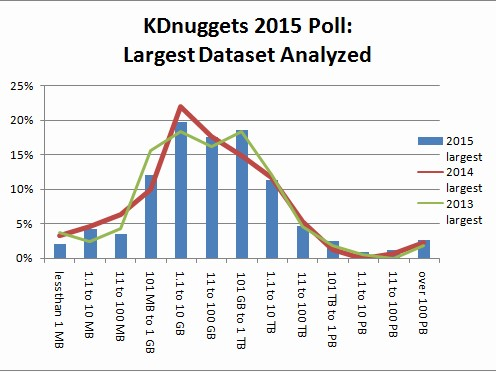
\includegraphics[width=\textwidth]{largest_dataset.jpg}
%{\footnotesize Encuesta: \textit{What was the largest dataset you analyzed?} \href{http://www.kdnuggets.com/2015/08/largest-dataset-analyzed-more-gigabytes-petabytes.html}{Fuente}}
%\end{frame}

\begin{frame}
\frametitle{¿Qué es el \textit{Machine Learning}?}

De la Wikipedia:
\begin{quote}
Machine learning is a subfield of \textbf{computer science} that evolved from the study of \textbf{pattern recognition} and computational learning theory in \textbf{artificial intelligence}.
In 1959, Arthur Samuel defined machine learning as a ``Field of study that gives \textbf{computers the ability to learn without being explicitly programmed}". Machine learning explores the study and construction of algorithms that can learn from and make predictions on data.
\end{quote}

Está íntimamente ligado con otras disciplinas.
\end{frame}

\begin{frame}[plain]
\begin{center}
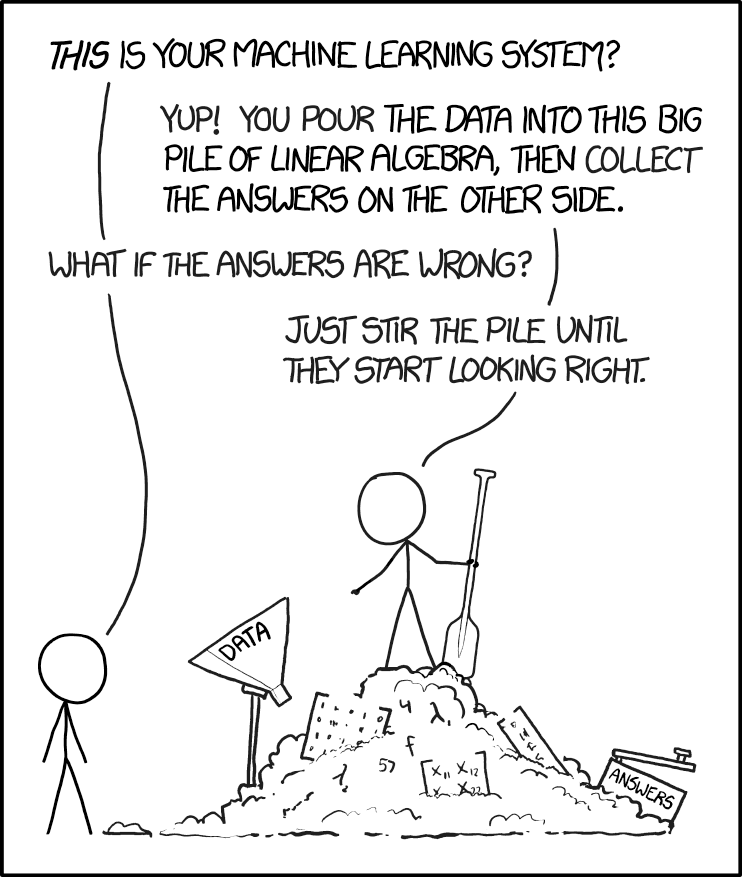
\includegraphics[height=0.85\textheight]{machine_learning_2x.png}

{\footnotesize \href{https://xkcd.com/1838/}{Fuente}}
\end{center}
\end{frame}

\begin{frame}[plain]
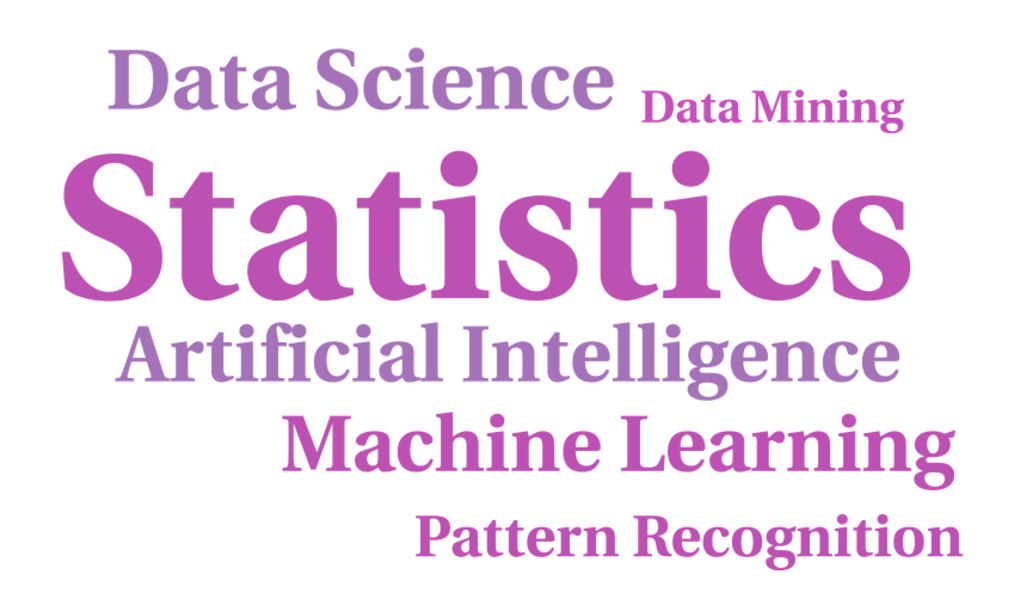
\includegraphics[width=\textwidth]{cloud.pdf}
\end{frame}

\begin{frame}[plain]
\begin{description}
\item[Statistics] Más antigua (aprox. 1749), el resto de disciplinas utilizan algunas de sus técnicas: estadística descriptiva, análisis de regresión, inferencia.
\item[Artificial Intelligence] Más moderna, 1940. Algunos problemas que intenta resolver: procesamiento lenguaje natural, planificación, visión por computador, robótica.
\item[Machine Learning] Rama de la IA, 1946. Se utiliza para resolver algunos de los problemas que tiene la IA.
\item[Pattern Recognition] En general se usa como sinónimo de \textit{Machine Learning}.
\item[Data Mining] Técnicas de modelado estadístico y \textit{machine learning} aplicadas a un dominio en concreto.
\item[Data Science] Término más moderno, mezcla de todo lo anterior.
\end{description}
\end{frame}

\begin{frame}
\frametitle{\textit{Data scientist}}

De la Wikipedia:
\begin{quote}
Data science employs techniques and theories drawn from many fields within the broad areas of mathematics, statistics, information science, and computer science, including signal processing, probability models, machine learning, statistical learning, data mining, database, data engineering, pattern recognition and learning, visualization, predictive analytics, uncertainty modeling, data warehousing, data compression, computer programming, artificial intelligence, and high performance computing.
\end{quote}

La conclusión es que se tratan de un perfil muy amplio, con un conjunto de habilidades poco definido.
\end{frame}


\begin{frame}
\frametitle{\textit{Data science} en la empresa}
\begin{itemize}
\item En 2012, Harvard Business Review publicó el artículo:

\begin{center}

\includegraphics[scale=0.4]{data.png}
\end{center}

\item La consultora \href{http://www.mckinsey.com/business-functions/business-technology/our-insights/big-data-the-next-frontier-for-innovation}{McKinsey} calcula que para 2018 habrá una demanda de entre 140,000-190,000 puestos de \textit{data science} sin cubrir.

\item Nadie sabe muy bien lo que es pero todo el mundo quiere uno.
\end{itemize}
\end{frame}


\begin{frame}
\frametitle{Flujo de trabajo de un equipo de \textit{data science}}
\begin{itemize}
\item En ocasiones un único perfil realiza todas las tareas.
\item Sin embargo, cada vez es más habitual tener un equipo donde cada integrante esté especializado en distintas partes del proceso. 
\end{itemize}
\begin{center}
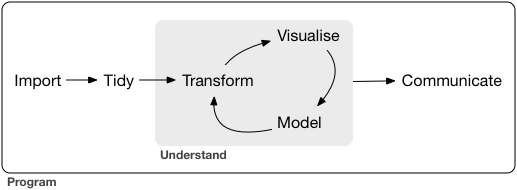
\includegraphics[width=0.85\textwidth]{data-science.png}

{\footnotesize Fuente: Hadley Wickham, \href{http://r4ds.had.co.nz/}{R for Data Science}}
\end{center}
\end{frame}

\begin{frame}[plain]
\frametitle{Herramientas de análisis}

\begin{center}
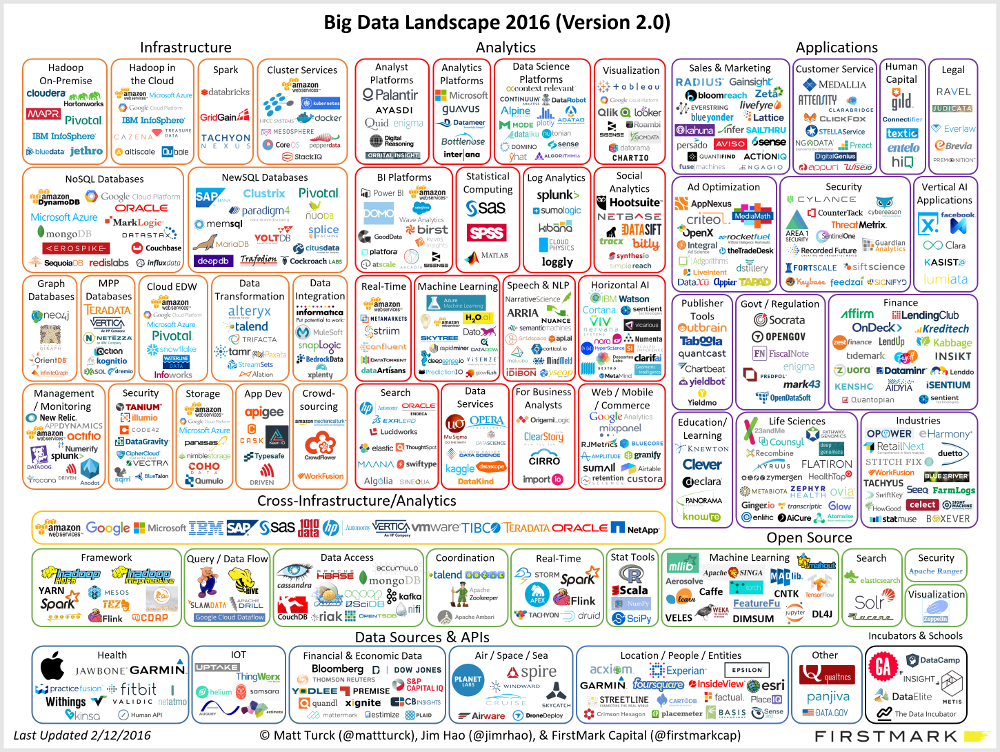
\includegraphics[width=\textwidth]{big_data_landscape.png}
\end{center}
\end{frame}


\begin{frame}[plain]
\begin{center}
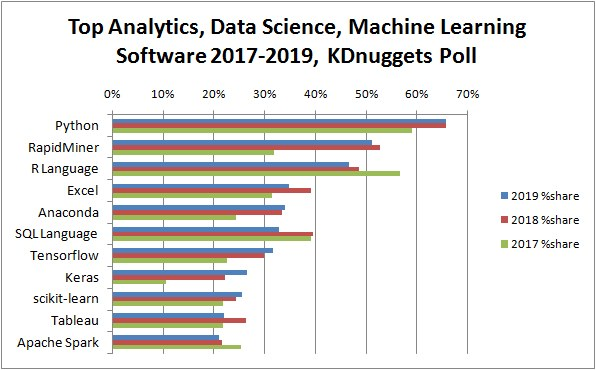
\includegraphics[height=0.75\textheight]{top-analytics-data-science-machine-learning-software-2019-3yrs-590.jpg}
\end{center}
{\footnotesize Software para proyectos de \textit{analytics}, y \textit{data science}. Encuesta de \href{https://www.kdnuggets.com/2019/05/poll-top-data-science-machine-learning-platforms.html}{KDnuggets}.}
\end{frame}


\begin{frame}
\frametitle{Algunas referencias}
\begin{enumerate}
\item Jerome H. Friedman. \textit{Data Mining and Statistics: What's the Connection?} (1998). \href{http://statweb.stanford.edu/~jhf/ftp/dm-stat.pdf}{[url]}
\item Leo Breiman. \textit{Statistical Modeling: The Two Cultures} (2001). \href{http://projecteuclid.org/download/pdf_1/euclid.ss/1009213726}{[url]}
\item Cross Validated.\textit{What is the difference between data mining, statistics, machine learning and AI?} (2010). \href{http://stats.stackexchange.com/questions/5026/what-is-the-difference-between-data-mining-statistics-machine-learning-and-ai}{[url]}
\item Sakthi Dasan Sekar. \textit{What is the difference between Artificial Intelligence, Machine Learning, Statistics, and Data Mining} (2014). \href{http://shakthydoss.com/what-is-the-difference-between-artificial-intelligence-machine-learning-statistics-and-data-mining/}{[url]}.
\item Cross Validated. \textit{What exactly is Big Data?} (2015). \href{http://stats.stackexchange.com/questions/173060/what-exactly-is-big-data}{[url]}
\item David Donoho. \textit{50 years of Data Science} (2015). \href{http://pages.cs.wisc.edu/~anhai/courses/784-fall15/50YearsDataScience.pdf}{[url]}
\end{enumerate}
\end{frame}


%\begin{frame}
%\frametitle{Análisis de datos}
%\begin{wideitemize}
%\item Es posible dividir el análisis de datos en dos tipos: generación de hipótesis y confirmación de hipótesis.
%\item Generalmente la generación de hipótesis se realiza mediante distintas visualizaciones y cálculo de estadísticos (exploración).
%\item Por otro lado, para confirmar una hipótesis se entrenan modelos estadísticos complejos.
%\item Esto no se cumple siempre: con un poco de cuidado se pueden utilizar visualizaciones para confirmar hipótesis y modelos para explorar unos datos. 
%\end{wideitemize}
%\end{frame}
%
%\begin{frame}
%\frametitle{Generación vs. confirmación de hipótesis}
%\begin{itemize}
%\item Para confirmar una hipótesis se deben de usar observaciones \textbf{independientes} de las que se han usado para generarla.
%\item Además, dichas observaciones no se pueden re-usar.
%\item De lo contrario, las conclusiones obtenidas serán demasiado optimistas.
%\item En la práctica, los datos se suelen dividir en dos conjuntos:
%\begin{enumerate}
%\item Conjunto de entrenamiento. Estos datos se pueden usar para explorar, ajustar múltiples modelos, etc.
%\item Conjunto de test. Una vez que nos hemos decidido por el modelo final y lo hemos ajustado, reportamos sus resultados en este sub-conjunto de los datos, que solo se puede usar \textbf{una} vez.
%\end{enumerate}
%\end{itemize}
%\end{frame}


\begin{frame}
\frametitle{Tipos de aprendizaje}

\begin{wideitemize}
\item \textbf{Supervisado}: dados pares de entrada-salida, el objetivo es inferir su relación \\
Ejemplos: regresión linea, regresión logística 

\item \textbf{No supervisado}: dados unos datos de entrada, el objetivo es inferir cierta estructura inherente en los mismos, sin necesidad de especificar las salidas de forma explícita\\
Ejemplos: clustering, reducción de dimensión

\item Existen otros tipos de tareas en los que el acceso a las salidas está limitado de distintas formas:
\begin{itemize}
\item Aprendizaje activo
\item Aprendizaje semi-supervisado
\item Aprendizaje por refuerzo
\end{itemize}
\end{wideitemize}
\end{frame}


\begin{frame}
\frametitle{Aprendizaje supervisado}

\begin{itemize}
\item Dado un conjunto de datos, compuesto por observaciones de diferentes variables, llamamos \textbf{variable respuesta} a aquella que es objeto del estudio.

\item Una vez identificada la respuesta, tenemos dos objetivos principales:

\begin{itemize}
\item Predicción: ser capaz de predecir cual va a ser la respuesta para observaciones futuras.
\item Información: extraer información sobre la relación de la variable de respuesta con el resto.
\end{itemize}

\item A su vez distinguimos dos tipos de problemas:

\begin{itemize}
\item Regresión: la variable respuesta es continua.
\item Clasificación: la variable respuesta es discreta (número finito de categorias).
\end{itemize}
\end{itemize}
\end{frame}


\section{Preproceso de datos}

\begin{frame}
\frametitle{Primeros pasos}

\begin{itemize}
\item Los datos a analizar a menudo provienen de fuentes variadas (redes sociales, sensores, encuestas, ...) y están almacenados en diferentes soportes (ficheros de texto, base de datos, ficheros binarios, \textit{streams}...).
\item Lo primero es identificar el problema qué queremos resolver y cuales son las variables que tenemos disponibles y pueden aportar información.
\item Ante la duda, no descartar variables/información ni observaciones antes de tiempo.
\item Lo segundo es combinar todas esa información y transformarla en una mezcla de variables numéricas (valores continuos) y categóricas (valores discretos).
\item El objetivo final del preproceso es organizar esos datos en un formato tabular (filas y columnas).
\end{itemize}

\end{frame}

\begin{frame}
\frametitle{Distintos tipos de información}

\begin{itemize}\addtolength{\itemsep}{\fill}
\item En ocasiones no es trivial transformar ciertos tipos de información en variables numéricas y/o categóricas.
\item Para estos casos a menudo es necesario un preproceso extra, muy dependiente del problema a resolver y específico del dominio.
\item Ejemplos típicos:
\begin{itemize}
\item Texto (tweets, páginas web, documentos): \textit{word2vec}, \textit{bag-of-words}, modelos \textit{n-gram}.
\item Imágenes: valores RGB de los píxeles, intensidad de gris.
\item Audio: transformada de Fourier, coeficientes MFCC.
\item Video: secuencia de \textit{frames}.
\end{itemize}
\end{itemize}
\end{frame}

%\begin{frame}[allowframebreaks]
%\frametitle{Ejemplo: MNIST}
%\begin{center}
%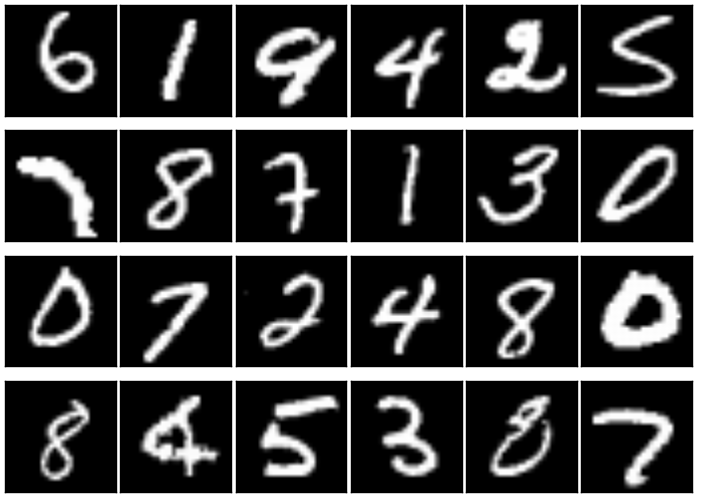
\includegraphics[width=0.85\textwidth]{mnist.png}
%
%{\footnotesize \href{http://yann.lecun.com/exdb/mnist/}{Base de datos MNIST}}
%\end{center}
%
%Cada dígito:
%\begin{itemize}
%\item se recorta
%\item se escala para que ocupe exactamente $20 \times 20$ píxeles.
%\item se centra en un recuadro de $28 \times 28$ píxeles.
%\end{itemize}
%Para transformarlo en datos tabulares:
%\begin{enumerate}
%\item consideramos cada imágen como una matriz de $28$ filas y $28$ columnas donde se almacenan los valores de 0 (negro) a 255 (blanco) de intensidad de gris.
%\item convertimos esa matriz un un vector muy largo de $28\times 28=784$ elementos.
%\item apilamos los vectores de los distintos números uno encima de otro.
%\end{enumerate}
%\end{frame}
%
%
%\begin{frame}
%\frametitle{\textit{Tidy data}}
%
%\begin{itemize} \setlength{\itemsep}{\fill}
%\item El 80\% del tiempo del análisis de datos se pasa limpiando y preparando datos (Dasu and Johnson 2003).
%
%\item Una vez cargados los datos, es conveniente estructurarlos de forma que el procesado posterior sea lo más sencillo posible.
%
%\item Una estructura muy común son los datos ordenados o \textit{tidy data}.
%
%\item Hadley Wickham (\href{http://vita.had.co.nz/papers/tidy-data.pdf}{2014}) los define como aquellos donde:
%
%\begin{enumerate}
%\item Cada variable forma una columna.
%\item Cada observación o muestra forma una fila.
%\item Cada tipo de unidad de observación forma una tabla.
%\end{enumerate}
%\end{itemize}
%\end{frame}


\begin{frame}
\frametitle{\textit{Missing values}}

\begin{itemize}
\item Es importante distinguir cuando una variable tiene valor $0$ ó no conocido.
\item Estos valores pueden venir representados por múltiples caracteres (``*", ``-", campo vacio, etc.).
\item Hay que codificarlos de manera especial para tenerlos en cuenta en los análisis.
\item En general,
\begin{enumerate}
\item Si tenemos suficientes datos, podemos simplemente ignorar las observaciones en las que falte alguno.
\item Sino, podemos completar dichas observaciones que faltan con, por ejemplo, la mediana del resto.
\end{enumerate}
\item \textbf{Ejemplo}: en datos que provienen de un reconocimiento médico varios pacientes no tienen ningún valor en el campo de ``Fármacos''. No toman ninguna medicación o el médico no ha registrado la respuesa?
\end{itemize}
\end{frame}

\begin{frame}
\frametitle{\textit{Outliers}}
\begin{wideitemize}
\item Distinguir si un valor es erróneo o válido pero extremo es muy complicado y dependiente del dominio.
\item Existen test estadísticos que permiten identificarlos.
\item En general no son perjudiciales, pero si es importante corregir los valores que son \textbf{imposibles}.
\item \textbf{Ejemplo}: en datos provenientes de un reconocimiento médico, aparece un paciente con un IMC de 50.
\end{wideitemize}
\end{frame}


\begin{frame}
\frametitle{Normalización}

\begin{itemize}
\item Las variables numéricas suelen tener rangos muy diversos.
\item Ejemplo: salario (1000 -- 1000000 \euro) y edad (0--100).
\item Algunos modelos interpretan esta diferencia de escalas como que unas variables son más importantes que otras.
\item Existen varias normalizaciones para que estas variables sean comparables:
\begin{itemize}
\item Media $0$ varianza $1$.
\item Escalar al intervalo $-1$, $1$.
\item ...
\end{itemize}
\item En ocasiones normalizar las variables también puede ayudar a que el proceso de aprendizaje sea más rápido.
\item Cuidado al analizar los resultados, ya que están en los nuevos rangos.
\end{itemize}
\end{frame}

\begin{frame}
\frametitle{Variables categóricas}

\begin{itemize}
\item Muy comunes en distintas fuentes de datos.
\item Importante tenerlas en cuenta para la fase de preproceso y análisis previo.
\item Muy pocos algoritmos son capaces de tratarlas directamente.
\item Por tanto, antes de pasar a la siguiente etapa (modelado) queremos convertirlas en numéricas.
\item La transformación donde se asigna a cada uno de sus valores un número entero no suele ser buena idea, ya que crea una relación artificial de orden y falsea las distancias.
\item Una forma es utilizar una codificación ``\textit{dummy}''.
\end{itemize}
\end{frame}

\begin{frame}
\frametitle{Ejemplo codificación ``\textit{dummy}''}

\begin{tabular}{cc}
\toprule
Edad & Sexo \\
\midrule
34 & H \\
18 & M \\
67 & M \\
21 & M \\
15 & H \\
\bottomrule
\end{tabular}
%
\hfill $\boldsymbol{\Longrightarrow}$ \hfill
%
\begin{tabular}{ccc}
\toprule
Edad & Es mujer? & Es hombre?\\
\midrule
34 & 0 & 1 \\
18 & 1 & 0 \\
67 & 1 & 0 \\
21 & 1 & 0 \\
15 & 0 & 1 \\
\bottomrule
\end{tabular}
\hspace*{0.4em}

\vfill
\begin{itemize}
\item Finalmente, podemos eliminar una de las dos nuevas variables puesto que están perfectamente correladas.

\item En general, para una variable categórica con $p$ valores añadimos $p-1$ variables nuevas.
\end{itemize}
\end{frame}

\begin{frame}
\frametitle{Otras codificaciones}
\begin{itemize}\setlength{\itemsep}{\fill}
\item Si en la semántica de la variable hay implícita una relación de orden: Puntuación \{baja, media, alta\} $\Rightarrow$ \{1,2,3\}.

\item Si hay relación de orden y no queremos falsear las distancias:\\
\vspace{1em}

\begin{tabular}{lrc}
\toprule
Mes & Día & Temp. \\
\midrule
Enero & 29 & 22.2 \\
Enero & 30 & 27.8 \\
Enero & 31 & 28.6 \\
Febrero &  1 & 26.1 \\
Febrero &  2 & 25.3 \\
\bottomrule
\end{tabular}
%
\hfill $\boldsymbol{\Longrightarrow}$ \hfill
%
\begin{tabular}{cc}
\toprule
Días desde 01/01 & Temp. \\
\midrule
29 & 22.2 \\
30 & 27.8 \\
31 & 28.6 \\
32 & 26.1 \\
33 & 25.3 \\
\bottomrule
\end{tabular}
\end{itemize}
\end{frame}


\begin{frame}[fragile]
\frametitle{Factores}
\begin{itemize}
\item Un factor es un tipo de dato que se utiliza para codificar valores categóricos, por ejemplo: \texttt{renta} = \{alta, baja, media\}.
\item Se crean con la función factor:
\begin{verbatim}
   > f <- factor(c("hombre", "mujer", "mujer"))
\end{verbatim}
\item Se pueden ver los niveles (valores distintos) con la función \texttt{levels()}:
\begin{verbatim}
   > levels(f)
   [1] "hombre" "mujer"
\end{verbatim}
\item Función \texttt{relevel()}: reordena los niveles del factor especificado, poniendo el nivel especificado de primero
\end{itemize}
\end{frame}

\begin{frame}
  \frametitle{Operaciones con factores}
  \begin{itemize}
    \item Función \texttt{cut()}: crea un factor dividiendo en rangos un vector numérico de acuerdo a unos puntos de corte
    \item Función \texttt{tapply()}: aplica una función a cada uno de los elementos de un vector, dividos en los distintos grupos de un determinado factor.
    \item Función \texttt{by()}: similar a la anterior, pero el objeto sobre el que se aplica la operación agrupada puede ser un \texttt{data.frame}.
    \item Función \texttt{aggregate()}: similar a \texttt{tapply()} pero devuelve un \texttt{data.frame} y acepta ``fórmulas''.
    \item Funciones \texttt{table()}, \texttt{prop.table()}, \texttt{margin.table()} y \texttt{xtabs()}: crear tablas de contingencia a partir de ciertos factores
  \end{itemize}
\end{frame}


\begin{frame}
\frametitle{Visualización}

\begin{itemize}
\item En ocasiones es útil hacer gráficos de algunas variables para ver que tipo de relación tienen con la respuesta.
\item Sin embargo, a medida que los conjuntos de datos son más grandes:
\begin{enumerate}
\item el número de variables puede ser muy grande, incluso del orden de millones.
\item la relación de las variables de entrada es muy compleja y altamente no lineal.
\end{enumerate}
\item En esos casos es muy difícil hacer gráficos que proporcionen información relevante, ya que podemos representar como mucho 2 o 3 dimensiones.
\item Los gráficos múltiples (facetas) y algunas transformaciones estadísticas (reducción de dimensionalidad) pueden aliviar el problema.
\end{itemize}
\end{frame}


\begin{frame}
\frametitle{Ejemplo}

\begin{center}
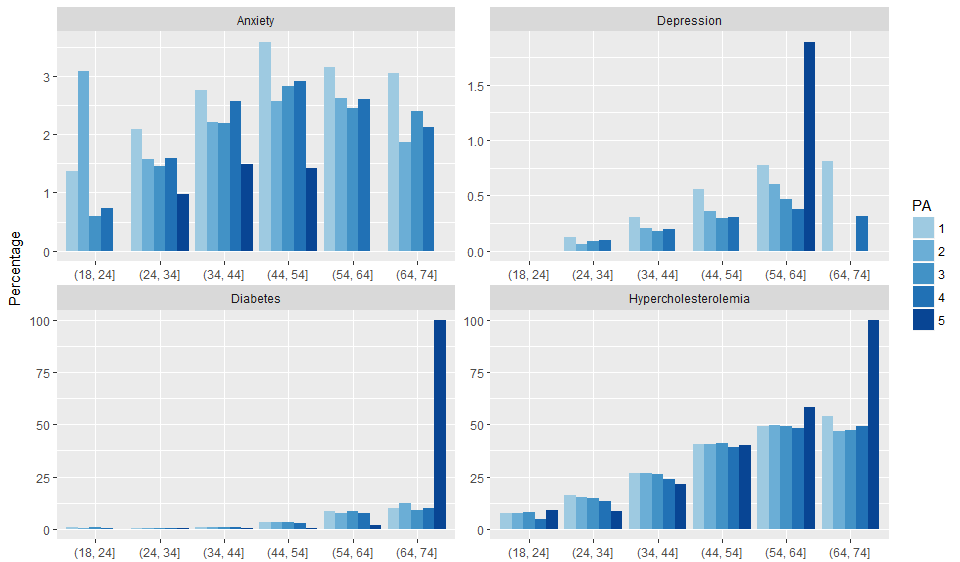
\includegraphics[width=\textwidth]{PA.png}
\end{center}

\end{frame}


\section{Modelos lineales básicos}

\subsection{Regresión lineal}

\begin{frame}
\frametitle{Regresión lineal: ejemplo}

\centering
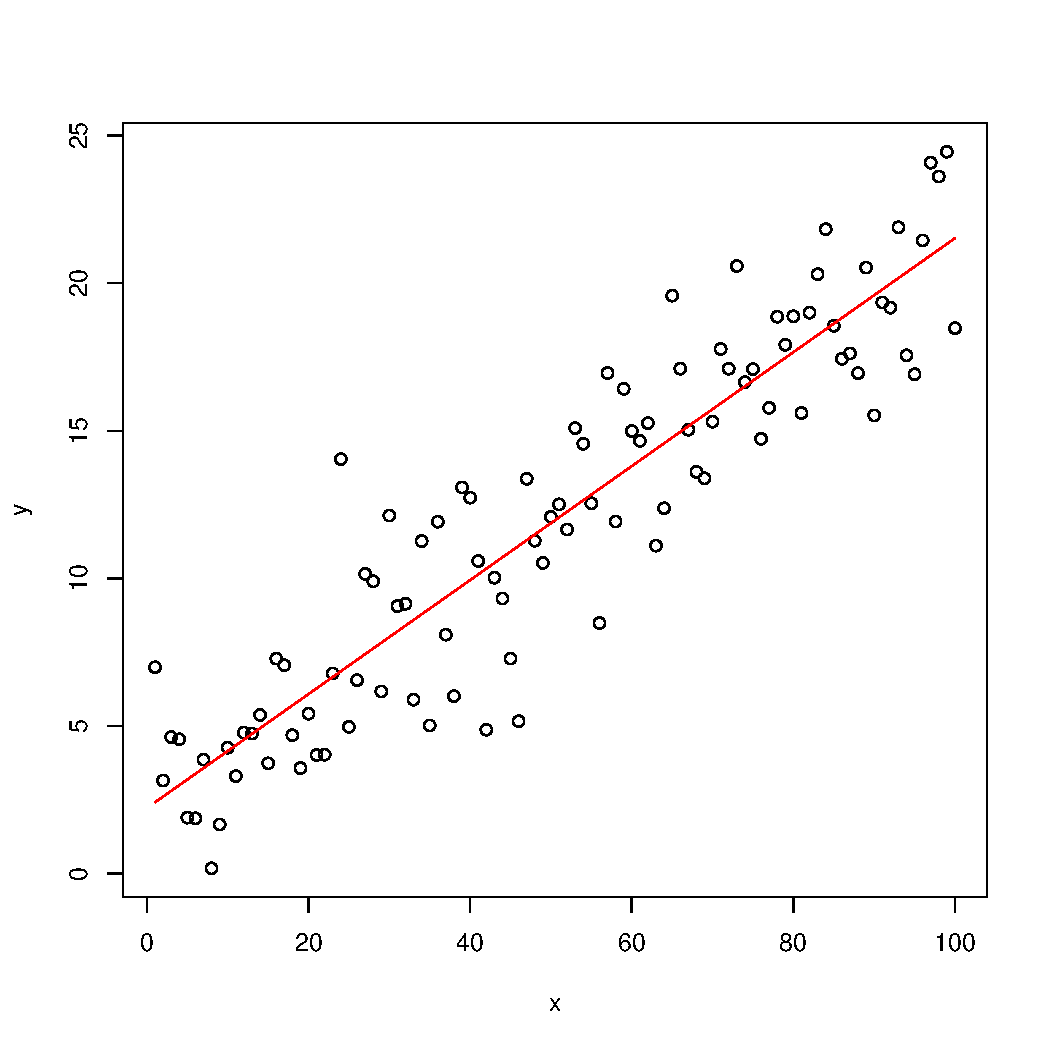
\includegraphics[width=0.7\textwidth]{linear_regression.pdf}
\end{frame}


\begin{frame}
\frametitle{Regresión lineal}

\begin{wideitemize}

\item La regresión linear asume que la variable de respuesta $y$ depende linealmente de las variables independientes,

$$y = w_0 + x_1w_1 + x_2w_2 + x_3w_3 + \dots + x_dw_d$$

\item Si tenemos $n$ observaciones de cada una de las variables, podemos escribirlo en notación matricial

$$\ybf = \Xbf\wbf$$

\item El término de bias $w_0$ se incluye como una columna constante de $1$s en $\Xbf$

\item El objetivo es estimar los pesos o coeficientes $w$
\end{wideitemize}
\end{frame}


\begin{frame}
\frametitle{Hipótesis de la regresión lineal}

\begin{wideitemize}
\item El método más común para calcular la recta de regresión se conoce como mínimos cuadrados.

%\item Consiste en una ``simple'' fórmula, y se puede aplicar para cualquier número de variables.

\item Teóricamente, para que el ajuste esté bien definido se asume que:
\begin{enumerate}
\item la respuesta depende linealmente de las variables
\item el modelo está especificado correctamente (no faltan variables)
\item hay menos variables que observaciones
\item no hay dos variables con correlación perfecta
\end{enumerate}

\item Es un modelo preditivo, ya que nos permite calcular el valor de $y$ para nuevos valores de $x$.

\end{wideitemize}
\end{frame}


\begin{frame}
\frametitle{Mínimos cuadrados}

\centering
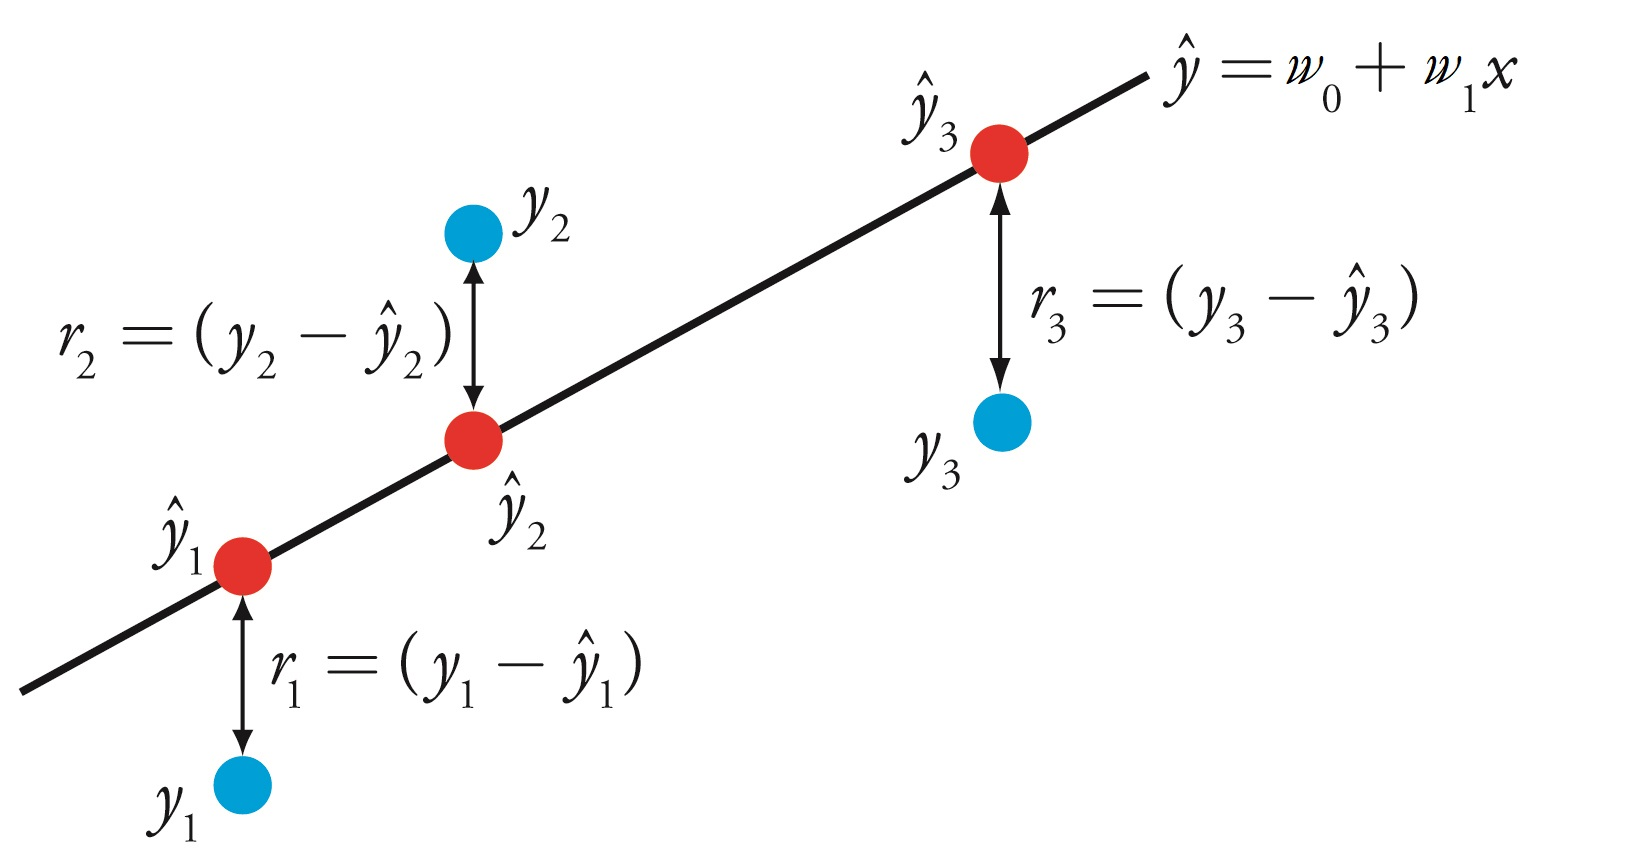
\includegraphics[width=\textwidth]{minimos_cuadrados.jpg}

\end{frame}



\begin{frame}
\frametitle{Cuarteto de Anscombe}

La pregunta es, ¿cómo de bien se ajusta la recta a nuestros datos?

\vfill
\centering
\hspace*{-1.5em}
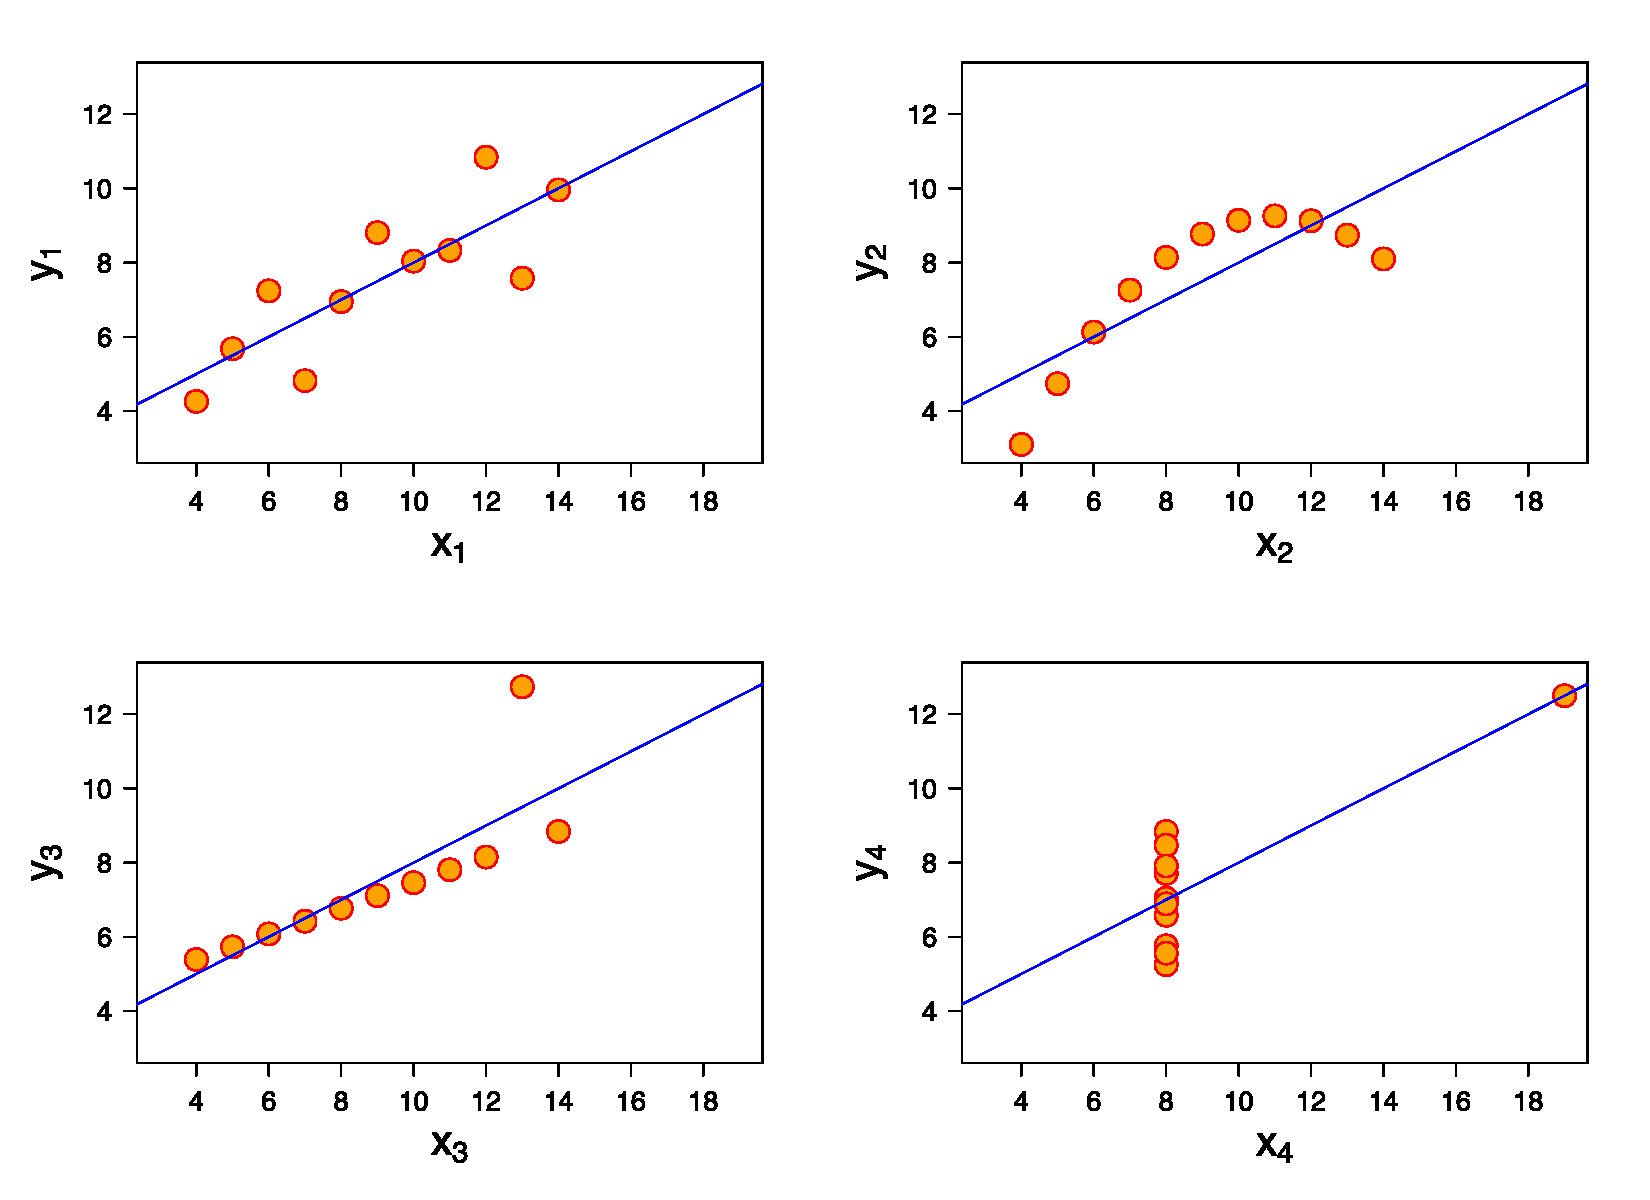
\includegraphics[width=0.8\textwidth]{anscombe.pdf}
\end{frame}


\begin{frame}
\frametitle{Bondad de ajuste}

\begin{wideitemize}
\item Históricamente se medía la calidad del modelo ó ``bondad del ajuste'' con diversos test sobre los residuos:
\begin{itemize}
\item Homocedásticos (varianza constante)
\item Media cero
\item Sin autocorrelación
\item (Distribución normal)
\end{itemize}

%\item Ya en 2001 Breiman cuestionaba si examinando los residuos se podía medir la aplicabilidad del modelo en cierta clase de problemas.

\item El módelo puede ser útil a pesar de que las hipótesis de la regresión y los test sobre los residuos no se cumplan.

\item A menudo nos interesa únicamente la \textbf{capacidad predictiva}.

\item ``\textit{All models are wrong, but some are useful}'' (George Box).
\end{wideitemize}
\end{frame}

\begin{frame}
\frametitle{Minimización del riesgo empírico}

\begin{itemize}
\item Necesitamos definir formalmente a que nos referimos con \textbf{capacidad predictiva}.

\item Dadas unas variables $\xbf$, queremos encontrar una función $f(\xbf)$ que se parezca lo máximo posible a la respuesta $y$.

\item Para ello, necesitamos una función de pérdida $L(f(\xbf), y)$ que cuantifique cuando de diferente es nuestra predicción del valor real.

\item El problema de aprendizaje consiste por tanto en encontrar la función $f$ que minimiza la pérdida media de todas las observaciones: $$\hat{f} = \argmin\; \frac{1}{n}\sum_{i=1}^{n}{L(f(\xbf_i), y_i)}$$
\end{itemize}
\end{frame}

\begin{frame}
\frametitle{Sobreajuste}

\begin{itemize}
\item Si resolvemos el problema anterior con el error cuadrático como función de pérdida $L(f(\xbf), y) = (f(\xbf)-y)^2$, obtenemos el estimador de mínimos cuadrados.

\item Por tanto, ya tenemos una forma de calcular el error de predicción de nuestro modelo original.

\item La pregunta ahora es, podemos mejorar el modelo (disminuir su error)?

\item Sí, aunque el modelo tiene que ser lineal en las variables, se pueden añadir nuevas variables que sean transformaciones polinómicas.

\item De hecho, siempre podemos añadir expansiones polinómicas de forma que el error sea casi $0$.
\end{itemize}
\end{frame}


\begin{frame}
\frametitle{Sobreajuste: ejemplo}
\centering
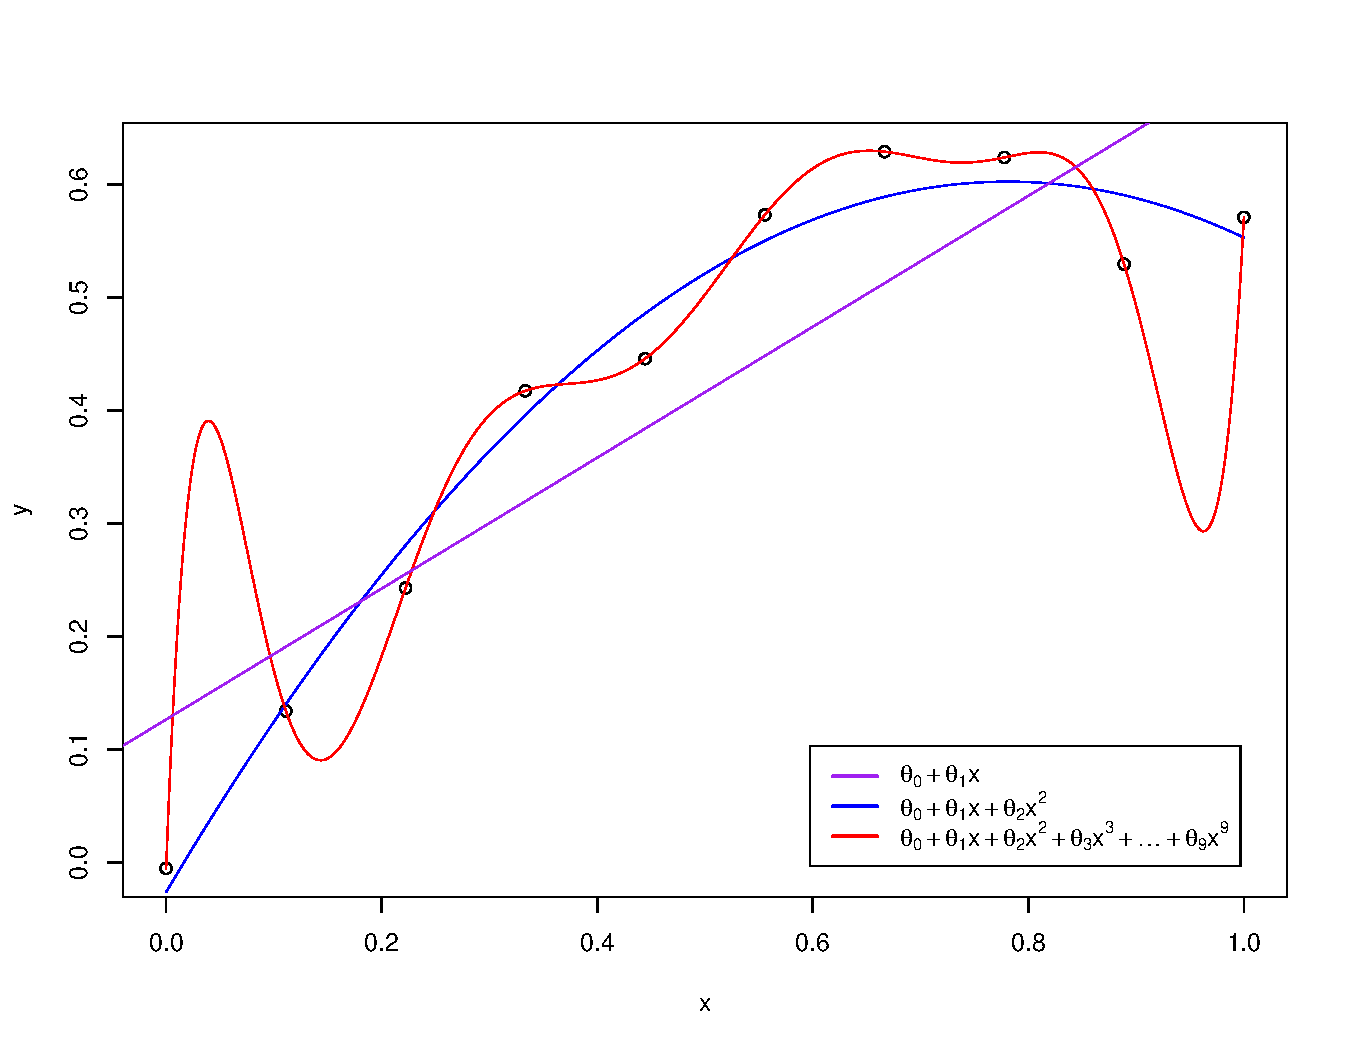
\includegraphics[height=0.85\textheight]{overfit1.pdf}
\end{frame}

\begin{frame}
\frametitle{Equilibrio sesgo-varianza: intuición}
\begin{itemize}
\item Si el modelo es muy simple, la solución esta sesgada y no ajusta bien los datos.
\item Si el modelo es muy complejo, es muy sensible a pequeños cambios en los datos.

\item En general el error calculado sobre las muestras usadas para entrenar el modelo (error de \textbf{entrenamiento}) es demasiado optimista.

\item El error de entrenamiento se puede hacer arbitrariamente pequeño aumentando la complejidad del modelo.

\item Nos interesa el error de \textbf{generalización}, es decir el error sobre muestras que el modelo no conoce.
\end{itemize}

\end{frame}

\begin{frame}
\frametitle{Equilibrio sesgo-variance: definición gráfica}
\centering
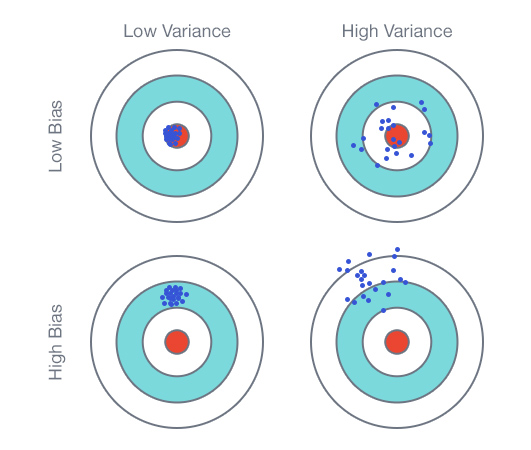
\includegraphics[height=0.80\textheight]{bias_variance_dardos.jpg}

{\footnotesize \href{http://blog.fliptop.com/blog/2015/03/02/bias-variance-and-overfitting-machine-learning-overview/}{Fuente}}
\end{frame}


\begin{frame}
\frametitle{Equilibrio sesgo-varianza: formulación}

El error teórico de predicción es
%
\begin{equation*}
\text{EP} = \Ebb[(y - \hat{f}(x))^2].
\end{equation*}
%
Se puede descomponer en
%
\begin{align*}
\text{EP} &= \underbrace{\Bigl(\Ebb[\hat{f}(x)] - f(x) \Bigr)^2}_{\text{Sesgo}^2}
           + \underbrace{E\Bigl[\hat{f}(x) - \Ebb[\hat{f}(x)] \Bigr]^2}_{\text{Varianza}}
           + \underbrace{\vphantom{\Bigl(}\sigma^2}_{\text{Ruido}}
\end{align*}
%
\begin{itemize}
\item Los términos de sesgo y varianza son opuestos: si disminuimos uno el otro aumenta y viceversa.
\item El término del ruido es inherente a los datos y no podemos hacer nada.
\end{itemize}
\end{frame}

\begin{frame}
\frametitle{Conjuntos de entrenamiento y test}

\begin{itemize}
\item En la práctica, lo primero que hacemos cuando cargamos unos datos es dividirlos aleatoriamente en dos subconjuntos, entrenamiento y test.
\item El subconjunto de test nos lo guardamos y no se utiliza \textbf{nunca} en la fase de aprendizaje del modelo.
\item Una vez construido el modelo, se comprueba su rendimiento en el conjunto de test.
\item Este último error es una buena estimación no sesgada de como se va a comportar nuestro modelo con nuevos datos.
\item Existe una gran probabilidad de sobreajuste si el error de test es muy alto en comparación con el error de entrenamiento.
\end{itemize}
\end{frame}

\begin{frame}
\frametitle{Error de predicción en función de la complejidad}
\centering
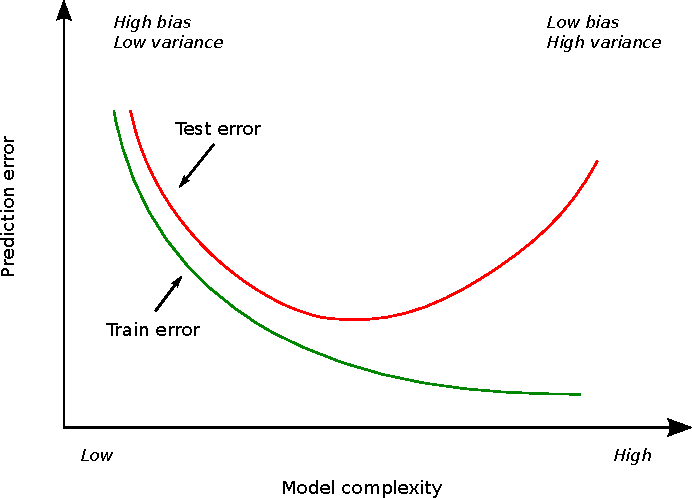
\includegraphics[height=0.75\textheight]{biasvariance.pdf}
\end{frame}


\begin{frame}
\frametitle{Errores de regresión}

Dado el valor real de la observación $i$, $y_i$ y la predicción del modelo $\hat{y}_i$, podemos calcular:

\begin{itemize}
\item MAE (Mean absolute error)

$$\text{MAE} = \frac{1}{n}\sum_{i=1}^{n}{|y_i - \hat{y}_i|}$$

\item MSE (Mean squared error)

$$\text{MSE} = \frac{1}{n}\sum_{i=1}^{n}{(y_i - \hat{y}_i)^2}$$

\end{itemize}
\end{frame}



\begin{frame}[fragile]
\frametitle{Modelos lineales en R}
\begin{itemize}
\item En R un modelo lineal de la variable de respuesta $y$ sobre las variables $x_1$, \dots, $x_d$, se define con la fórmula $$y \sim x_1 + x_2 + \dots + x_d$$
\item Para ajustar un modelo lineal por mínimos cuadrados se usa la función \texttt{lm()}, pasando como primer argumento la fórmula anterior.
\item Las fórmulas también pueden contener expresiones aritméticas de variables (expansiones polinómicas, logaritmos, etc).
\item Ejemplo: modelo de regresión de la variable \texttt{mpg} sobre \texttt{wt}

\begin{Verbatim}[commandchars=\\\{\}]
   > fit <- lm(mpg \mytilde wt, data=mtcars)
\end{Verbatim}
\end{itemize}
\end{frame}


\begin{frame}[fragile]
\frametitle{Fórmulas}
\begin{itemize}
\item Las fórmulas son objetos especiales de R que respresentan relaciones simbólicas entre variables:

\texttt{respuesta \mytilde\  variables independientes}

\item Se usan en funciones como \texttt{aggregate()}, \texttt{boxplot()}, y \texttt{lm()}.

\item Los operadores aritméticos tienen otro significado cuando se usan dentro de las fórmulas. Ejemplos:

\begin{Verbatim}[commandchars=\\\{\}]
   y \mytilde u + v + w + u:v + u:w + v:w
   y \mytilde u * v * w - u:v:w
   y \mytilde (u + v + w)^2
\end{Verbatim}

\item Si queremos que tengan su significado habitual tenemos que utilizar el operador \texttt{I()}:
\begin{Verbatim}[commandchars=\\\{\}]
   y \mytilde u + v + w + I(u*v) + I(u*w) + I(v*w)
\end{Verbatim}
\end{itemize}
\end{frame}


\begin{frame}
\frametitle{Ejercicio regresión}
Con el conjunto de datos \texttt{diamonds}:
\begin{itemize}
\item Separarlos aleatoriamente en un 60\% de entrenamiento y un 40\% de test.
\item Ajustar un modelo lineal del precio sobre los quilates.
\item Ajustar un modelo cuadrático con las mismas variables.
\item Calcular el error cuadrático medio sobre el conjunto de entrenamiento y test, definido como $$\text{ECM} = \frac{1}{n}\sum_{i=1}^{n}{(y_i - \hat{y}_i)^2},$$ donde $y$ es la variable respuesta y $\hat{y}$ la predicción del modelo.
\item ¿Qué pasa ahora si ajustamos el modelo sobre todas las variables? ¿Disminuye el error?
\end{itemize}
\end{frame}


\subsection{Regresión logística}

\begin{frame}
\frametitle{Regresión logística}

\begin{wideitemize}
\item Es un modelo lineal para problemas de clasificación.
\item En lugar de una variable continua, la respuesta es ahora una variable discreta con $2$ o más valores, que se denominan \textit{clases}.
\item En el caso binario, el modelo estima la probabilidad de que cada uno de los ejemplos pertenezca a la clase $0$ o $1$.
\item Finalmente se predice la clase $0$ si la probabilidad es menor que $0.5$ y la clase $1$ en caso contrario.
\item Se puede ver como una caso especial del modelo lineal generalizado.
\end{wideitemize}
\end{frame}

\begin{frame}
\frametitle{Regresión logística: formulación}

\begin{wideitemize}
\item La fórmula de la regresión logística es
$$y = \sigma(w_0 + w_1x_1 + w_2x_2 + ... + w_dx_d)$$
donde $\sigma(\cdot)$ es la función logística
$$\sigma(t) = \frac{1}{1 + e^{-t}}$$

\item La función logística siempre tiene como salida un número en el intervalo $(0, 1)$

\item Por tanto, interpretamos la salida del modelo como la probabilidad de pertenecer a una clase o a la otra (clasificación binaria)

\end{wideitemize}
\end{frame}


\begin{frame}
\frametitle{Regresión logística: ejemplo}
\centering
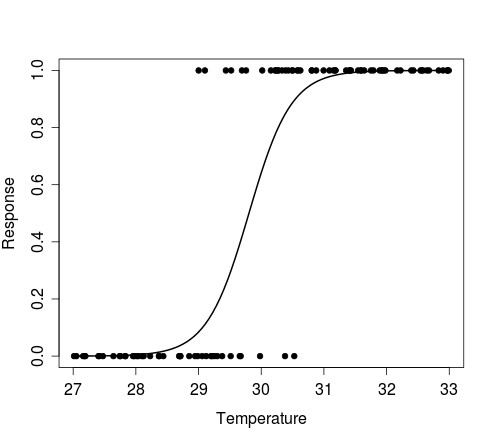
\includegraphics[height=0.85\textheight]{log_reg.png}
\end{frame}


\begin{frame}
\frametitle{Interpretación de coeficientes: odds ratio}
\begin{itemize}
\item Dado un modelo lineal con una única variable independiente, el odds ratio se define como

$$\text{OR} = \frac{\exp(w_0 + w_1(x+1))}{\exp(w_0 + w_1x)} = \exp(w_1)$$

\item Es decir, como cambian las probabilidades de la salida cuando la variable $x$ aumenta una unidad:
\begin{itemize}
\item Si $\text{OR}=1$ la variable $x$ no tiene ninguna asociación con la salida
\item Si $\text{OR}>1$ la variable está asociada con una mayor probabilidad de la salida
\item Si $\text{OR}<1$ la variable está asociada con una menor probabilidad de la salida
\end{itemize}
\end{itemize}
\end{frame}


\begin{frame}
\frametitle{Errores de clasificación}

Los principales errores de clasificación se pueden calcular a partir de la \textbf{matriz de confusión}:
\vfill
\begin{columns}[T] % align columns
\begin{column}{.40\textwidth}
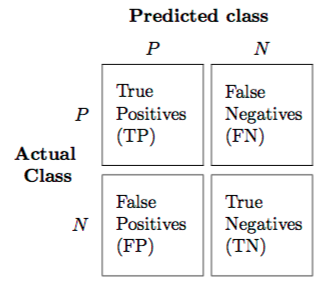
\includegraphics[scale=0.5]{confusion_matrix.png}
\end{column}%
\hfill%
\begin{column}{.56\textwidth}
\begin{wideitemize}
\item[] Accuracy: $\frac{\text{TP} + \text{TN}}{\text{P} + \text{N}}$

\item[] Sensitivity, recall, TPR: $\frac{\text{TP}}{\text{TP} + \text{FN}}$

\item[] Specificity, TNR: $\frac{\text{TN}}{\text{TN} + \text{FP}}$

\item[] Precision, PPV: $\frac{\text{TP}}{\text{TP} + \text{FP}}$

\item[] F1 score: $2\times \frac{\text{PPV} \times \text{TPR}}{\text{PPV} + \text{TPR}}$
\end{wideitemize}
\end{column}%
\end{columns}
\end{frame}


\section{Extensiones}

\subsection{Modelos lineales generalizados (GLM)}

\begin{frame}
\frametitle{Modelos lineales generalizados (GLMs)}

\begin{wideitemize}
\item Generalización de la regresión lineal que permite distribuciones de errores distintas de la distribución normal.

\item Se asume que la media de dicha distribución depende de las variables independientes de la siguiente forma:
$$\Ebb(\ybf) = \mu = g^{-1}(\Xbf\wbf)$$
donde $\Ebb(\cdot)$ es el valor esperado y $g$ es la función de enlace

\item La función de enlace proporciona la relación entre la media de la distribución y el predictor lineal
\end{wideitemize}
\end{frame}


\begin{frame}
\frametitle{Ejemplo: distribución de Bernoulli}

\begin{wideitemize}
\item Cuando la distribución de la salida $\ybf$ es una Bernoulli el modelo se conoce con el nombre de regresión logística

\item La función de media es la logística,

$$\mu = g^{-1}(\Xbf\wbf) = \frac{1}{1 + \exp(-\Xbf\wbf)}$$

\item La función de enlace es la inversa de la anterior,

$$\Xbf\wbf = g(\mu) = \ln\left(\frac{\mu}{1 - \mu}\right)$$

\item Para cada distribución, hay una función de enlace ``canónica'' que es la que se usa habitualmente
\end{wideitemize}

\end{frame}


\begin{frame}
\frametitle{Ejemplo: distribución de Poisson}

\begin{wideitemize}
\item Esta distribución está indicada cuando queremos modelizar una variable de salida entera y no real (por ej. conteos)

\item Función de media

$$\mu = \exp(\Xbf\wbf)$$

\item Función de enlace

$$\Xbf\wbf = \ln(\mu)$$

\item Otras distribuciones posibles son la Gamma, Exponencial, Multinomial, etc.
\end{wideitemize}
\end{frame}


\begin{frame}[fragile]
\frametitle{GLMs en R}
\begin{wideitemize}
\item La función para ajustar modelos lineales generalizados es \texttt{glm()}
\item Tiene los mismos argumentos principales que \texttt{lm()}, pero además tenemos que especificar la distribución de la variables dependiente con el parámetro \texttt{family}
\item Ejemplo: regresión logística

\begin{Verbatim}[commandchars=\\\{\}]
   > fit <- glm(Species \mytilde Petal.Length, data=iris, 
                family=binomial)
\end{Verbatim}
\item Por defecto se usa la función de enlace ``canónica'', pero esto se puede modificar (ver ayuda)
\end{wideitemize}
\end{frame}


\subsection{Regularización}

\begin{frame}
\frametitle{Regularización}

\begin{itemize}
\item El estimador de mínimos cuadrados para la regresión lineal es el \textit{mejor} estimador no sesgado, donde \textit{mejor} se refiere al que tiene menor varianza.

\item Sin embargo, a menudo se puede reducir esta varianza bastante, en detrimento de introducir un pequeño de sesgo.

\item Esto se consigue limitando la complejidad del modelo con un término de \textbf{regularización}.

\item Un ejemplo muy común es Ridge Regression, que añade una regularización $l_2$ a mínimos cuadrados:
$$\min_\wbf\;||\Xbf\wbf - \ybf||^2_2 + \lambda||\wbf||^2_2$$

\end{itemize}
\end{frame}


\begin{frame}
\frametitle{Lasso}

\begin{itemize}
\item Similar a Ridge Regression, Lasso añade un término de regularización $l_1$:

$$\min_\wbf\;||\Xbf\wbf - \ybf||^2_2 + \lambda||\wbf||_1$$

donde 
$$||\wbf||_1 = \sum_{i=1}^{d}{|w_i|}$$

\item El valor absoluto promueve que muchos coeficientes sean $0$ después de ajustar el modelo

\item Dichos coeficientes no tienen por tanto efecto en la salida

\item Se podría considerar que son variables ``poco importantes''
\end{itemize}
\end{frame}


\begin{frame}
\frametitle{Elastic Net}

\begin{itemize}
\item Combina las regularizaciones de Ridge y Lasso:
$$\min_\wbf\;||\Xbf\wbf - \ybf||^2_2 + \lambda_1||\wbf||_1 + \lambda_2||\wbf||_2^2$$

\item Otra forma de escribirlo:

$$\min_\wbf\;||\Xbf\wbf - \ybf||^2_2 + \lambda(\alpha||\wbf||_1 + (1 - \alpha)||\wbf||_2^2)$$

\item Para $\alpha = 0$ recuperamos Ridge Regression y para $\alpha = 1$ el Lasso

\item Mantiene la dispersión en los coeficientes del Lasso pero en general se obtienen mejores modelos en términos de error

\item Problema: tenemos que decidir el valor de dos hiper-parámetros ($\alpha$ y $\lambda$)
\end{itemize}
\end{frame}


\begin{frame}
\frametitle{Paquete \texttt{glmnet} y \texttt{glmnetUtils}}

\begin{wideitemize}
\item Implementa GLMs con regularización Lasso y Elastic Net

\item Muy eficiente (escrito en Fortran)

\item Se pueden ajustar no solo regresiones lineales con regularización, sino también regresiones logísticas, regresiones de Poisson, etc.

\item Implementa también un mecanismo para seleccionar automáticamente el parámetro $\lambda$ (pero no $\alpha$) usando validación cruzada

\item \texttt{glmnet} no tiene interfaz para fórmulas, pero \texttt{glmnetUtils} incorpora una

%\item Para más información cargar el paquete y escribir \texttt{?glmnet}
\end{wideitemize}
\end{frame}


\begin{frame}[allowframebreaks]
\frametitle{Ejercicio titanic}

Vamos a intentar predecir la supervivencia de las víctimas del Titanic a partir de las siguientes variables:

\begin{itemize}
\item \texttt{survival}:  Supervivencia (0 = No; 1 = Si)
\item \texttt{pclass}:   Clase de pasajero (1, 2, 3)
\item \texttt{name}:      Nombre
\item \texttt{sex}:           Sexo
\item \texttt{age}:          Edad
\item \texttt{sibsp}:           Número de hermanos/esposos/as a bordo.
\item \texttt{parch}:          Número de padres/hijos a bordo
\item \texttt{ticket}:          Número de ticket
\item \texttt{fare}:         Coste del billete
\item \texttt{cabin}:          Cabina
\item \texttt{embarked}:        Puerto de embarque
\end{itemize}

\break

\begin{enumerate}
\item Cargar el fichero \texttt{titanic.csv} en R.
\item Ver cuantos valores \textit{missing} tiene cada variable con \texttt{summary}.
\item Eliminar la variable \texttt{Cabin} (¿por qué?).
\item Eliminar también las variables \texttt{PassengerId}, \texttt{Name} y \texttt{Ticket} (¿por qué?).
\item Eliminar las filas que contengan algún \texttt{NA} (función \texttt{na.omit}).
\item Convertir la variable \texttt{Survived} a un factor.
\item Dividir datos en 80\% \texttt{entrenamiento} y 20\% \texttt{test}, aleatoriamente.
\item Ajustar un modelo de regresión logística estándar y otro con regularización (función \texttt{glm} y paquete \texttt{glmnet}).
\end{enumerate}
\end{frame}

\subsection{Modelos aditivos generalizados (GAM)}
\begin{frame}
\frametitle{Modelos aditivos generalizados (GAM)}

\begin{itemize}
\item Extensión de los GLMs donde la salida depende linealmente de funciones de las variables predictoras:
%
$$\Ebb(y) = g^{-1}(f_1(x_1) + f_2(x_2) + f_3(x_3) + ... + f_d(x_d))$$

\item Las funciones pueden ser distintas para cada una de las variables

\item Pueden ser paramétricas o funciones generales ``suaves''

\item La mayoría de implementaciones modernas restringen las funciones para que sean de la forma

$$f_i(x_i) = \sum_{k=1}^{K_i}\beta_{ik}b_{ik}(x_i)$$

donde $b_{ik}(x_i)$ son funciones de base

\end{itemize}
\end{frame}


\begin{frame}[fragile]
\frametitle{Paquete \texttt{mgcv}}

\begin{wideitemize}
\item Implementación de GAMs en R, alternativa al clásico paquete \texttt{gam}

\item Varias funciones de suavizado posible

\item Incluye el grado de ``suavizado'' en el ajuste del modelo (no es necesario especificarlo)

\item Incluye múltiples distribuciones (Binomial, Bernoulli, Poisson, etc.)

\item Ejemplo:
\begin{Verbatim}[commandchars=\\\{\}]
   > fit <- gam(mpg \mytilde s(wt), data=mtcars)
\end{Verbatim}

\end{wideitemize}

\end{frame}


\begin{frame}
\frametitle{Ejercicio}
Con los datos de diamantes del ejercicio anterior:
\begin{itemize}
\item Ajustar un GAM del precio sonbre los quilates
\item Comparar el error sobre el conjunto de test con el modelo lineal y con el modelo lineal añadiendo una nueva variable que sea el cuadrado del precio

\item Ajustar un modelo Lasso modelizando el precio usando el resto de variables de entrada
\item ¿Cuál es el valor del lambda óptimo?
\item ¿Qué variables son las más importantes y cuales son innecesarias?
\end{itemize}
\end{frame}


\section{Análisis de resultados}

\begin{frame}
\frametitle{Diseño iterativo}

\begin{wideitemize}
\item Si el resultado del modelo no es tan bueno como nos gustaría no hay que perder la esperanza, ya es muy común que el análisis se realize de forma iterativa.
\item Podemos probar varias cosas:
\begin{enumerate}
\item Ajustar mejor el modelo: muchos de los modelos que hemos visto tienen parámetros que influyen mucho en el rendimiento (más a continuación).
\item Probar otros modelos: una opción muy común al hacer el análisis de unos datos es comenzar con modelos más simples e ir moviéndonos hacia modelos más complejos.
\item Obtener más datos: no siempre es posible, pero en general con más datos se consigue mejor resultado que un algoritmo más inteligente.
\end{enumerate}
\end{wideitemize}
\end{frame}

\begin{frame}
\frametitle{Conjunto de validación}
\begin{itemize}
\item Para escoger los valores de los parámetros de un modelo, podemos mirar el error de entrenamiento para varios valores y escoger el de menor error.
\item Al hacer esto, hemos visto que el error de entrenamiento es una medida sesgada y por tanto los valores de los parámetros pueden no funcionar bien en el conjunto de test.
\item Por tanto, necesitamos un tercer conjunto llamado conjunto de \textbf{validación} donde se va a medir el error para cada valor de los parámetros.
\item Finalmente, escogemos el que tenga menor error de validación.
\item El conjunto de test sigue sin tocar, y se usa como antes para estimar el error de generalización.
\end{itemize}
\end{frame}

\begin{frame}
\frametitle{Validación cruzada}
\begin{itemize}
\item Si no tenemos muchos datos y no queremos hacer un conjunto de validación, podemos usar validación cruzada.
\end{itemize}

\begin{center}
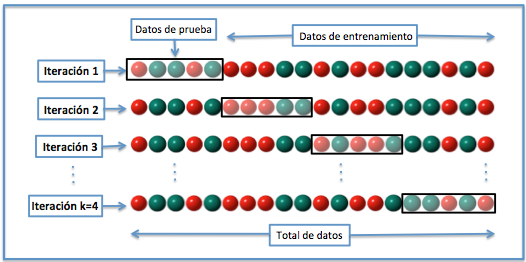
\includegraphics[width=1\textwidth]{crossval.jpg}

{\footnotesize \href{https://commons.wikimedia.org/w/index.php?curid=17616792}{Fuente}}
\end{center}
\end{frame}

\begin{frame}
\frametitle{Selección de variables y reducción de dimensión}

\begin{itemize}
\item Una forma de reducir el tiempo de computación de los algoritmos de aprendizaje es reduciendo el número de variables.
\item Esto se puede hacer de dos maneras:
\begin{enumerate}
\item Seleccionando únicamente un subconjunto de las variables de acuerdo a algún criterio de relevancia para predecir la respuesta.
\item Proyectando nuestros datos a un espacio de menor dimensión.
\end{enumerate}
\item La primera opción tiene la ventaja de que las variables siguen siendo interpretables, es decir, tienen significado semántico.
\item El método más común de proyección es PCA o análisis de componentes principales.
\end{itemize}
\end{frame}


\begin{frame}
\frametitle{Colecciones de paquetes útiles}
\begin{itemize}
\item En \href{https://support.rstudio.com/hc/en-us/articles/201057987-Quick-list-of-useful-R-packages}{este} enlace se puede ver una lista muy reciente de paquetes útiles.
\item \href{https://cran.r-project.org/web/views/MachineLearning.html}{Machine Learning in R} es una colección de paquetes de aprendizaje automático.
\item \href{http://cran.r-project.org/web/views/HighPerformanceComputing.html}{High-Performance computing in R} es una colección de paquetes de útiles para la computación de alto rendimiento.
\item Recientemente aplicaciones web que permiten la visualización de resultados también gozan de gran popularidad, por ejemplo los notebooks de \href{http://jupyter.org/}{Jupyter}.
\item En R destaca \href{http://shiny.rstudio.com/}{Shiny}, que permite convertir código R en aplicaciones web interactivas.
\end{itemize}
\end{frame}

\begin{frame}
\frametitle{Paquetes más populares de ML}
\centering
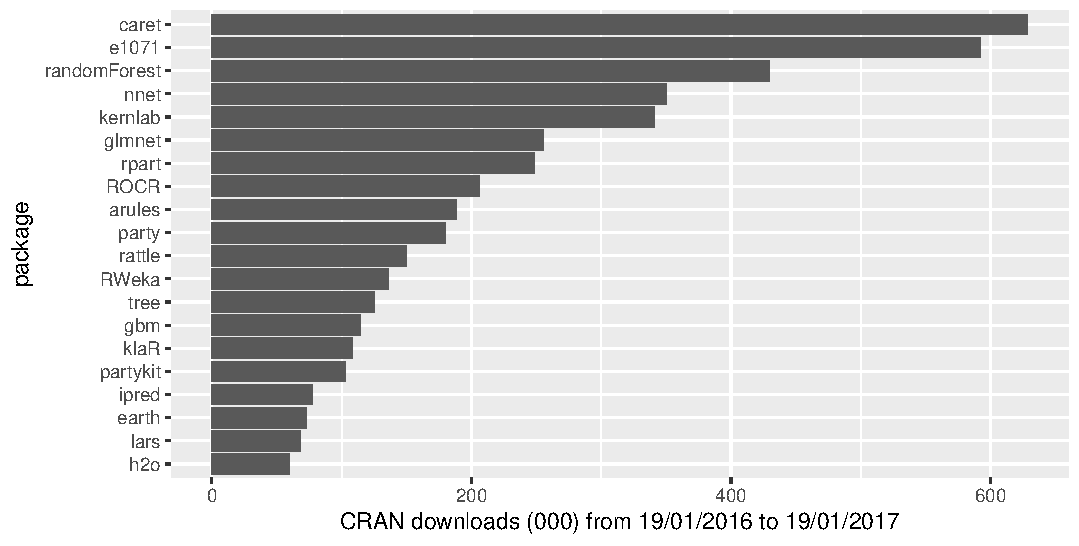
\includegraphics[width=\textwidth]{top20.pdf}

{\footnotesize Descargas Enero 2016 - Enero 2017. \href{https://github.com/thedataincubator/data-science-blogs}{Fuente}}
\end{frame}


\begin{frame}
\frametitle{Resumen paquetes destacados}
\begin{itemize}\addtolength{\itemsep}{0.3\baselineskip}
\item Modelos lineales y utilidades:
\begin{itemize}
\item \texttt{caret}, utilidades para clasificación y regresión
\item \texttt{MASS}, ridge regression
\item \texttt{ridge}, ridge regression con selección automática del hiper-parámetro
\item \texttt{glmnet}, GLMs con regularización Lasso o Elastic Net
\item \texttt{glmnetUtils}, utilidades para \texttt{glmnet}
\item \texttt{gam}, modelos aditivos generalizados
\item \texttt{mgcv}, modelos adictivos generalizados (recomendado)
\end{itemize}
\item Algunos modelos más complejos:
\begin{itemize}
\item \texttt{nnet}, Redes neuronales, también regresión logística multinomial
\item \texttt{e1071}, Support Vector Machines
\item \texttt{gbm}, Gradient Boosting
\item \texttt{randomForest}, Random Forest
\item \texttt{xgboost}, Extreme Gradient Boosting
\end{itemize}
\end{itemize}
\end{frame}


\begin{frame}
\frametitle{\textit{Tidyverse}}

\begin{itemize}
\item Conjunto de paquetes creados por Hadley Wickham que comparten una misma API y contienen funciones para el análisis de datos:
\begin{itemize}
    \item \textbf{\texttt{ggplot2}}, para hacer gráficos avanzados.
    \item \textbf{\texttt{dplyr}}, para manipular datos.
    \item \textbf{\texttt{tidyr}}, para limpiar datos.
    \item \textbf{\texttt{readr}}, para importar datos.
    \item \texttt{purrr}, para programación funcional.
    \item \texttt{tibble}, implementa \textit{tibbles}, una versión moderna de los data.frames.
\end{itemize}

\item El paquete \textit{tidyverse} instala y carga los paquetes anteriores.

\item También instala otros paquetes que pueden ser útiles aunque no los carga por defecto.

\item Para más información y la lista completa de paquetes: \url{https://github.com/tidyverse/tidyverse}.
\end{itemize}
\end{frame}


\begin{frame}
\frametitle{Libros y manuales}

En general, se pueden encontrar muchos manuales en las secciones \textit{Manuals} y \textit{Contributed} de \href{https://cran.r-project.org/}{CRAN}, así como ejemplos en la web \href{https://rpubs.com/}{RPubs}. Algunos recursos más específicos:

\begin{description}
\item[Libros]
\begin{itemize}
 \item R for Data Science \href{http://r4ds.had.co.nz/}{[url]}.
 \item An Introduction to Statistical Learning with Applications in R \href{http://www-bcf.usc.edu/~gareth/ISL/}{[url]}.
\end{itemize}
\item[E-Books]
\begin{itemize}
\item YaRrr! The Pirate's Guide to R \href{http://nathanieldphillips.com/thepiratesguidetor/}{[url]}.
\item The R Inferno \href{http://www.burns-stat.com/pages/Tutor/R_inferno.pdf}{[url]}.
\item R Programming \href{https://en.wikibooks.org/wiki/R_Programming}{[url]}.
\end{itemize}
\item[Blogs]
\begin{itemize}
\item RTutorial \href{http://www.r-tutor.com/}{[url]}.
\item Quick-R \href{http://www.statmethods.net/}{[url]}.
\item RStudio \href{https://blog.rstudio.org/}{[url]}.
\item RBloggers \href{https://www.r-bloggers.com/}{[url]}.
\end{itemize}
\end{description}

\end{frame}

\begin{frame}
\frametitle{FAQs y comunidades}
\begin{itemize}
\item \href{http://stackoverflow.com/questions/tagged/r}{StackOverflow}: las preguntas con el tag R contienen mucha información y problemas resueltos. Además, las nuevas preguntas se responden en cuestión de horas.

\item \href{http://stats.stackexchange.com/}{CrossValidated}: no es una comunidad específica de R (más bien de estadística), pero hay mucha información acerca de cómo realizar procedimientos concretos de análisis de datos y aprendizaje automático en R.

\item \href{https://twitter.com/RLangTip}{@RLangTip}: Twitter que publica consejos y trucos diarios.

\item \href{https://plus.google.com/u/0/communities/115516770321395255377}{R Programming for Data Analysis}: Comunidad de Google+.
\item \href{https://plus.google.com/u/0/communities/117681470673972651781}{Statistics and R}: Otra comunidad de Google+.
\item \href{https://www.linkedin.com/grp/home?gid=77616}{The R Project for Statistical Computing}: Grupo de LinkedIn.
\end{itemize}
\end{frame}

\end{document}
